\documentclass[conference,compsoc]{IEEEtran}
\usepackage{ifpdf}
\usepackage{caption}
\usepackage[pdftex]{graphicx}
\usepackage[noadjust]{cite}
\usepackage{amsmath}
\usepackage[caption=false,font=footnotesize,labelfont=sf,textfont=sf]{subfig}
\usepackage{fixltx2e}
\hyphenation{op-tical net-works semi-conduc-tor}
\renewcommand{\citedash}{--}


\begin{document}

\title{Visual Dataflow Language for Educational Robots Programming}

\author{
	\IEEEauthorblockN{Grogorii Zimin}
	\IEEEauthorblockA{
		Mathematics and Mechanics Faculty,\\
		SPbSU\\
		Saint-Petersburg, Russia \\
		Email: zimin.grigory@gmail.com
	}
	
	\and

	\IEEEauthorblockN{Dmitrii Mordvinov}
	\IEEEauthorblockA{
		Mathematics and Mechanics Faculty,\\
		SPbSU\\
		Saint-Petersburg, Russia \\
		Email: mordvinov.dmitry@gmail.com
	}
}

\maketitle



\begin{abstract}
REWRITE THIS SH..
The paper describes dataflow visual programming language based on DSM-approach. Its purpose is to be bridge between lightweight robotics languages for education and complex industrial languages. A short review of programming languages for robots is presented here. Also different approaches and architectures for developing control system for robots are considered. For demonstration of language usage, the paper provide solution for creating control system of robot based on subsumption architecture. 
\end{abstract}

\section{Introduction}

Programming languages for creating robotic controllers are actual topics of research oftenly discussed at major conferences, such as ICRA\cite{Icra} or IROS\cite{Iros2016}. Visual programming languages (VPLs) are also actively discussed for the last three decades, the largest conferences are held annually, e.g. VL/HCC\cite{VLHCC}. VPLs are oftenly applied in robotics domain\cite{banyasad2000visual,simpson2006mobile,simpson2008visual,posso2011process,diprose2011ruru} allowing to create and visualize robotic controllers. Robotic VPLs are commonly used for educational purposes, making possible for students of even junior schools to create robotic programs. There already exists a great number of educational robotic programming environments based on VPLs, e.g. NXT-G\cite{nxtg}, TRIK Studio\cite{trik}, ROBOLAB\cite{robolab}, also there are some academic tools implementing interesting and novel approaches to educational robotics programming\cite{banyasad2000visual,simpson2008visual,diprose2011ruru}.

Robotic control programs are inherently reactive: they transform data which is continuously coming from multiple sensors into the impulses on actuators. For this reason dataflow languages (DFLs) are well-suitable for robotics programming. Many researchers denoted the conveniency of dataflow visual programming languages (DFVPLs)\cite{johnston2004advances}, finding them more useful than textual DFLs, for example because data flows explicitly displayed on the diagram. There are large and complex general-purpose and domain-specific development environments such as LabVIEW\cite{labview} and Simulink\cite{simulink} that provide a large (and sometimes even cumbersome) set of libraries for robotics programming. More detailed discussion of robotics VPLs will be provided in section~\ref{sec:Overview}.

There is a large number of robotic constructor kits for learning the basics of robotics and cybernetics, such as LEGO MINDSTORMS\cite{legokit}, TRIK, ScratchDuino\cite{http://www.scratchduino.com/}. Modern programming languages that are used for programming those kits are based on the control flow model rather than on dataflow model. Control flow-based languages are good for solving scholar ``toy'' tasks, but may be inconvenient for programming more complex ``real world'' controllers that may be conveniently expresses on DFLs. The simple DFVPL may be considered as a useful step from educational VPLs to the programming languages that are used in unversities and industry. 


%In SPbSU cybernetic laboratory are conducted a number of studies aimed at improving the tools for design and programming of embedded systems for small robot platforms (e.g. LEGO, TRIK) using block diagrams\cite{}. Goal of research paper is the development of novel extensible tool for programming all small robot platforms which discussed above in dataflow style. While dataflow approach is commonly used approach when each element is executing in separate thread or process. Our approach avoids it, because it brings a large overhead on target platforms, details presented in section~\ref{sec:lang}. There are several commonly used robots controller architectures: Connell's Colony, Maes' Action-Selection, Arkin's Motor Schema, Rosenblatt's Distributed Architecture for Mobile Navigation, Brooks' Subsumption Architecture\cite{simpson2009toward}. DFLs are suitable for Brooks' Subsumption Architecture, his approach are commonly used\cite{banyasad2000visual,simpson2006mobile,posso2011process,proetzsch2007behaviour}. So, our approach also uses Brooks’ Subsumption Architecture as the fundamental concept used in the our DFVPL.

This paper discusses a novel extensible tool for programming all popular educational robotic kits on dataflow visual programming language. One of the most important distinction of our tool from others is its focus on embedded systems (sec.~\ref{sec:Implementation}). Another interesting detail of our work is the application of DSM-aproach for implementation of visual editor: it is entirely generated by QReal DSM-platform\cite{qrealMeta}\cite{kuzenkova2013qreal} without even a line of code written. We also take into consideration the popularity of Brooks' Subsumption Architecture\cite{brooks1986robust} which is still mainstream aproach to design of complex robotic controllers\cite{banyasad2000visual,simpson2006mobile,posso2011process,proetzsch2007behaviour} despite it was proposed 30 years ago. Brooks’ Subsumption Architecture and some other are conveniently expressed in our language, they are discussed in sec.~\ref{}.

The remainder of a paper is organized as follows. An overview of robotics VPLs and DFVPLs is presented in section~\ref{sec:Overview}. A description of our language is given in section~\ref{sec:lang}. Section~\ref{sec:example} demonstrates two typical robotic controllers expressed in our language. The most important details of implementation are deiscussed in section~\ref{sec:Implementation}. Finally, the last section concludes the paper and discusses possible directions for future work.


\section{Similar Tools}
\label{sec:Overview}
Robot programming environments can be divided into three categories: educational, which allows to program small educational robotic kits; industrial, which have a rich toolkit for creating large and complex robotic controllers; academic, which implement new interesting ideas, however they are oftenly unavailable for downloading or unusable.

Educational visual enviroments are for example NXT-G and ROBOLAB for LEGO MINDSTORMS NXT kit, EV3 Software for the Lego Mindstorms EV3 kit, TRIK Studio for NXT, EV3 and TRIK. Those environments simplify solving primitive robot control tasks like finding a way out of the maze and driving along the line using light sensors, which makes the process of learning the basics of programming and robot control easy. But their simplicity oftenly bounds the flexibility of the language. Visual languages of all mentioned systems are based on control flow model.

There is also a number of well-known visual robotic programming environments of industrial level. For example, general-purpose LabVIEW from National Instruments with the DFVPL G, programming environment Simulink developed by MathWorks for modeling different dynamic models or control systems. Those products offer to a huge set of models and libraries to create control systems, test benches, real-time systems of any complexity, using model-driven approach. LabVIEW provides opportunity for programming small robots. There are lots of examples of applying LabVIEW in education\cite{erwin2000lego, 1_gomez-de-gabriel_mandow_fernandez-lozano_garcia-cerezo_2011}, but much more oftenly its adaptations like Robolab are used in educational process. It should be noted that those environments are distributed under the commercial license.

Another example of an visual robotics industrial system is the Microsoft Robotics Developer Studio (MSRDS)\cite{jackson2007microsoft}, which is free for academic purposes and allow to create distributed robotic systems on DFVPL. MSRDS officially supports a large set of robotic platforms, LEGO NXT\cite{kim2007programming} in particular (however, the autonomious mode for NXT is not supported). MSRDS has the ability of manual integration with custom robotic platforms, but unhappily is not maintained since 2014.

There is a lot of scientific research done in this area, e.g., dissertation\cite{banyasad2000visual} describes a visual programming module for expressing robotic controllers in terms of extended Moore machines, \cite{simpson2008visual},\cite{posso2011process} describe visual environment for $occam\mbox{-}\pi$ language and $Transterpreter$ framework, and its usage in education and swarm robotics. Article\cite{diprose2011ruru} describes DFVPL for beginners which is pretty close to a one we introduce here. However at the moment RuRu is under development, it has pretty limited functionality and even unavailable for download.

% Нужна секция с архитектурами! Не забыть дополнить конец введения!
%There are several commonly used robots controller architectures: Connell's Colony, Maes' Action-Selection, Arkin's Motor Schema, Rosenblatt's Distributed Architecture for Mobile Navigation, Brooks' Subsumption Architecture\cite{simpson2009toward}. 


\section{DFVPL}
\label{sec:lang}
Evolution of a domain-specific modeling (DSM) methodology allows to quickly create a fairly sophisticated visual programming languages\cite{DSM}. TRIK Studio programming environment is an example of a system that was created using DSM-based approach on QReal platform\cite{qrealMeta, kuzenkova2013qreal}. Based on industrial experience of TRIK Studio developers, it had been decided to create the DFVPL based on QReal platform. We based our DFVPL on the several basic requirements.

\begin{itemize}
\item Brooks’ Subsumption Architecture should easily be expressed by means of language.
\item Robots behaviour diagram, as well as in TRIK Studio, should be have the opportunity to be interpreted on the two-dimensional simulation model of the robot or directly on robot via wi-fi.
\item Interpretation  of robots behaviour diagram  should emulate data flow common model, avoiding the strategy "one thread per block", but provides ability to manually create threads.
\end{itemize}


\subsection{Description of the blocks}
DFVPL block (element) is a entity which processes incoming on its channels data, and can emits result (or new data) on their output channels. Our DFVPL blocks can be divided into several groups.

\begin{itemize}
\item \textit{Control}. Blocks implementing design: conditions, loops, etc.
\begin{itemize}
\item \textit{Flow} implementing data transmission between others blocks (uses for connecting channels of blocks).
\item \textit{Fork, EndFork}. Blocks provide ability to force threading works.
\item \textit{RandomValue, ConstValue} Blocks are responsible for sending a random number or a predetermined value of any type.
\item \textit{GetSetVariable}. Pseudo DF block, which set value for given variable or emit it.
\item \textit{Loop, If, Switch}. These blocks implement common essence in DF style. \textit{Loop} is a custom entity which emitting the numbers or dummy data corresponding to predetermined settings. \textit{If} checks predetermined condition substituting variables by incoming data, and sends them to \textit{True} or \textit{False} channel. \textit{Switch} successively checks multiple conditions and if its evaluate as \textit{true} sends incoming data to corresponding channel.  	
\item \textit{Function} Block, which allows to make the processing of the input data in text language (PL Lua\cite{lua}), its support inherited from the code base of TRIK Studio). Most often, this block will be used for specifying mathematical operations on data.
\item \textit{FinalBlock} stops the execution of program, when receiving any data. 
\item \textit{SubprogramCall} is used to take out repetitive blocks on a separate diagram, and then use it as one block for data processing.
\item \textit{Wait} is simple block, which main goal is to delay data.
\item \textit{DelayFilter} is the evolution of the previous block, which add condition filtering and checking the number of emitted data validated by condition.
\end{itemize} 
\item \textit{Drawing}. Blocks for drawing on robots display and on the floor.
\begin{itemize}
\item \textit{Pen} is initialization block for drawing a predetermined color marker on the floor.  It controls the lowering and raising of the marker
\item \textit{PaintSettings} is block which used for define color of pen, background, width of the brush for drawing on robots display.
\item \textit{ShapePainter, SmilePainter, Text} are used for drawing some shape or text or smile on robots display. 
\item \textit{Clear} is block which clear robot display when receiving any data.
\end{itemize} 
\item \textit{Flow manipulation}. These elements provide opportunity to manipulate data which flow between blocks.
\begin{itemize}
\item \textit{InPort, OutPort}. Their purpose is the connecting incoming data to \textit{Subprogram} block and blocks which should received these data in it, and similarly from blocks in \textit{Subprogram} to output channels of \textit{Subprogram}. 
\item \textit{Supressor, Inhibitor} block or substitute data which flow via \textit{Flow}. These blocks and \textit{SubprogramCall} block provide support for the Brooks' Subsumption Architecture. 
\item \textit{Interflowing, Separator} provide opportunity to gather data from several \textit{Flows} into one and vice versa.
\end{itemize} 
\item \textit{Actions}. Blocks implements any actions which robot can make.
\begin{itemize}
\item \textit{Servo, Motors} process received data and send impulses to robot actuators.
\item \textit{Encoders} block sets the number of motor revolutions, when receiving data, and continuously emits current number for corresponding channels.
\item \textit{MessageToRobot, ReceiveMsg} responsible for the coordination of a group of robots. Sends data to specified robot via \textit{MessageToRobot}, and receive from any robots via \textit{ReceiveMsg}.
\item \textit{Say, PlayTone, Led} responsible for managing of sound and LED lights.
\item \textit{RemoveFile, WriteToFile} implement functions to working with files. \textit{WriteToFile} writes incoming data to specified file. \textit{RemoveFile} removes specified file or file which name it got from incoming data.
\item \textit{InitCamera, DetectByVideo, StreamingNode} provide access to all opportunities of video vision of TRIK controller: detect different objects and send data corresponding to specified (by incoming data or manually) object, stream video.
\item \textit{PortBlock} provides opportunities to write on some ports corresponding to robot device and emits data from it.
\item \textit{Sensor} continuously emits data from specified sensor, e.g. infrared, light, etc.
\item \textit{SystemCall} responsible for the command execution got from incoming data, e.g. "reboot" will reboot robot.
\item \textit{Gamepad} reads data from the control device, e.g. gamepad, and emits it.
\end{itemize} 
\end{itemize} 


One of the distinguishing features of our DFVPL is that some blocks are a single object on the diagram, and although it can be represented on the diagram in several places, only one of them works. It is modification of data flow paradigm which helps to work with our DFVPL as control flow VPL. For example figure~\ref{image:encoder} shows diagram with \textit{Motors, ConstValue, Encoders, Flows} where \textit{Encoders} block is presented twice. 

\begin{figure}[ht]
	\centering
	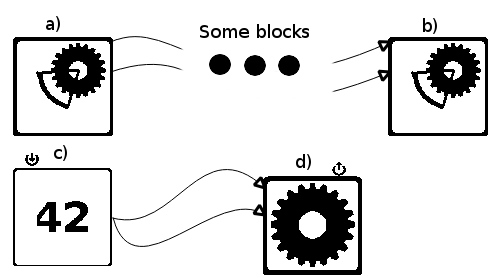
\includegraphics[width=3.5in]{Encoders.png}
	\caption{Block with many representations but only one of them can be active. a,b --- \textit{Encoders} c --- \textit{ConstValue} d --- \textit{Motors}}
	\label{image:encoder}
\end{figure}

When interpretation started \textit{ConstValue} emits data to \textit{Motors} and \textit{Encoders} (a) emits number of motor revolutions. After "Some blocks" \textit{Encoders} (b) receiving some data, which reinitialized block, at that moment \textit{Encoders} (a) stop emitting data (implementation details discussed in section~\ref{sec:impl}).

Let's describe some basic thing about our blocks. On figure~\ref{image:encoder} \textit{ConstValue} and \textit{Motors} have incoming and outgoing "arrows" to block, which are used to connect control flow data, e.g. \textit{Motors} emits data to control flow channel when handle incoming data, and \textit{ConstValue} emits its value when receive control flow data. On left, right and bottom side may be placed incoming and outgoing channels (points where \textit{Flows} may be pinned), which are signed when user edits block (see Figure~\ref{image:block}).
\begin{figure}[ht]
	\centering
	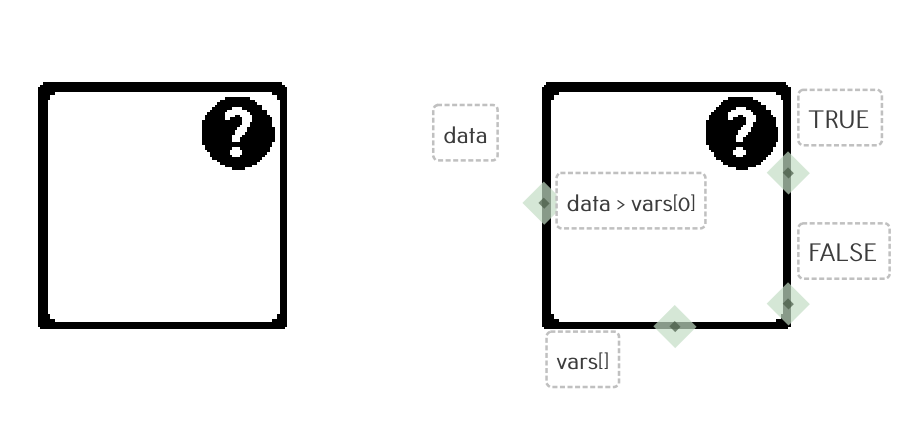
\includegraphics[width=3.5in]{block.png}
	\caption{Showing and editing of block.}
	\label{image:block}
\end{figure}
Also block may contain field for text, e.g. on Figure~\ref{image:block} user wrote condition.



These blocks are enough to control the robot and create varying complexity robot controllers, e.g. Figures~\ref{image:boxC},~\ref{image:box} show simple robot controller which control moving around box. Here we initialize some variables and regulate motors power based on the data continuously received from the infrared sensor. More complex, but typical robotic controller presented in section~\ref{sec:robotControl}. 

\begin{figure}[ht]
	\centering
	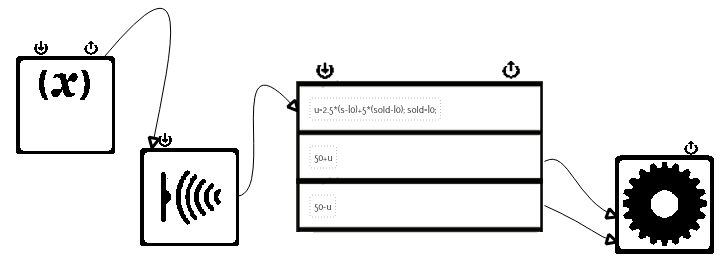
\includegraphics[width=3.5in]{alongBoxCode.png}
	\caption{Controller code for along box moving.}
	\label{image:boxC}
\end{figure}

\begin{figure}[ht]
	\centering
	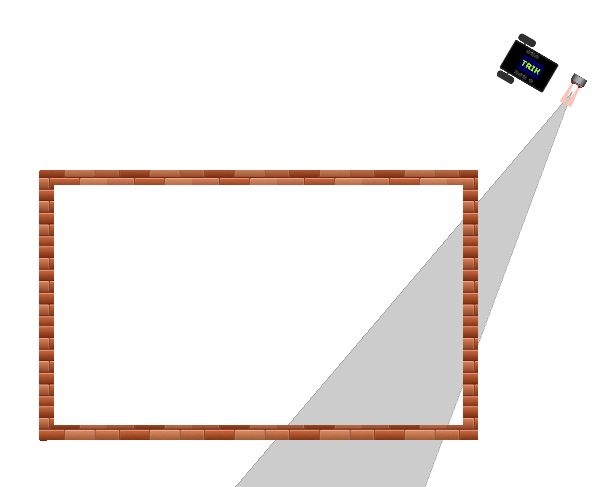
\includegraphics[width=3.5in]{alongBoxModel.png}
	\caption{Modelling of along box moving.}
	\label{image:box}
\end{figure}



\subsection{Pseudo dataflow}
The main direction of our language and programming tool is the small robots programming, so it was necessary to avoid the use of commonly used dataflow paradigm, when for each execution block created new thread or process. This method is perfect for larger and more complex robots equipped with powerful multi-core controllers. But for small robots linear increase in the number of blocks in the diagram will eventually reduce performance due to the overhead of thread- or process-switching.

So, our dataflow idiom was implemented as pseudo parallelism (see details in section~\ref{sec:impl}). But it is also exist opportunity to manually manage threads with two blocks --- \textit{Fork, EndFork}.

\section{Example}
\label{sec:example}
%Рассмотрим задачу управления движением робота при помощи джойстика, при условии, что робот сам избегает лобовых столкновений с припятствиями. Предполагается, что программа пишется для двухколесного мобильного робота, оборудованного спереди инфракрасными датчиками расстояния, для управления колесами используются силовые моторы.

%Разобьем задачу на два уровня поведения. Первый будет отвечать за обслуживание запросов пользователя. Второй будет ответственен за избегание столкновений: если робот близок к столкновению, то он должен уклониться от препятствия вне зависимости от того, что нажимает пользователь на пульте. 

%Рассмотрим первый уровень (рис.~\ref{image:layer1}). Пользователь управляет роботом посредством джойстика. Джойстик генерирует данные, соответствующие нажатиям кнопок или манипулирований рычагом направления. Для простоты считаем, что нажатие любой кнопки завершит программу управления роботом. Данные с рычага преобразуются блоком текстового программирования в соответствующие импульсы моторов робота, которые в данном случае передаются <<заглушкам>>, которые связаны с выходными портами блока <<Подпрограмма>>. 
%\begin{figure}[ht]
%	\centering
%	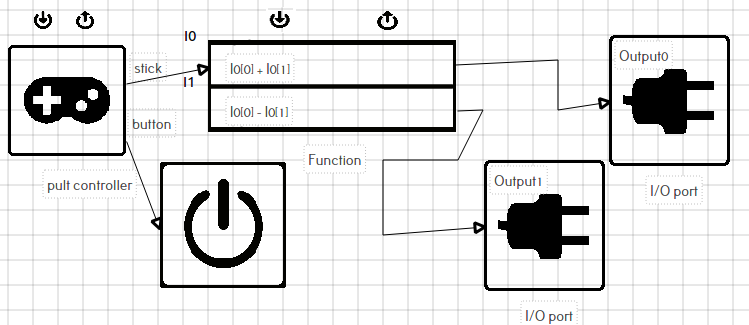
\includegraphics[width=3.5in]{pultLayer.png}
%	\caption{Уровень управления с пульта.}
%	\label{image:layer1}
%\end{figure}

%Рассмотрим второй уровень (рис.~\ref{image:layer2}): данные с датчиков расстояния собираются в вектор и передаются фильтру, который при опасности столкновения отправляет данные дальше в блок математической обработки (если условие не выполнилось, управление может быть передано по потоку <<ошибки>>, в данной программе этот поток не указан; также между проверками условия приходящие данные не обрабатываются (теряются) в течение установленного пользователем времени). В блоке математической обработки вычисляется мощность, которую необходимо подать на 2 мотора. Вычисленные значения передаются выходным портам.
%\begin{figure}[ht]
%	\centering
%	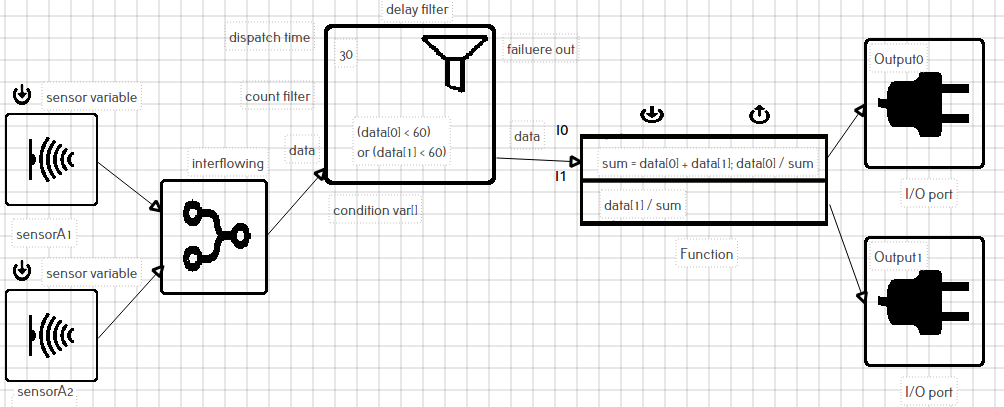
\includegraphics[width=3.5in]{collisionLayer.png}
%	\caption{Уровень избегания столкновений.}
%	\label{image:layer2}
%\end{figure}

%\begin{figure}[ht]
%	\centering
%	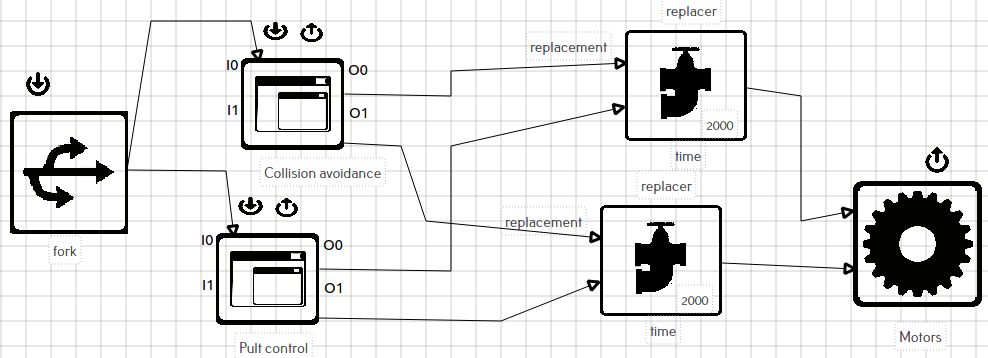
\includegraphics[width=3.5in]{programScreen.png}
%	\caption{Программа управления роботом.}
%	\label{image:prog}
%\end{figure}

%Имея два поведения, создаем управление роботом в модели Брукса (рис.~\ref{image:prog}). С помощью блока распараллеливания запускаем уровни поведения. Каждый уровень генерирует данные, соответствующие мощностям моторов, передаваемые на блок управления силовыми моторами. Так как второй уровень ответственности должен не позволить столкнуться с препятствием, его значения подавляют значения, полученные с первого уровня, с помощью блоков <<Подавления>>.

\section{Implementation}
\label{sec:Implementation}
The system is implemented as two plugins for TRIK Studio. The first one describes the visual language and provides visual editor for our system. It contains the metamodel of dataflow visual language and entirely generated by QReal DSM-platform. Plugged into TRIK Studio this module provides fully operational visual editor with all advantages of TRIK Studio control flow editor like modern-looking user interface, ability to create elements with mouse gestures, different appearances of links and so on. The time spent on the development of this plugin (not considering discussing and designing the prototype of visual language on paper) roughly equals three man-days. The benefit on exploiting the DSM-aproach is obviuos, the development of the similar editor from scratch would have been taken vastly more time.

The second plugin contains implementation of dataflow diagrams interpreter. Given the program drawn in editor (provided by first plugin) interpreter will transform that program into a sequence of the commands sent to a target robot (see fig.~\ref{image:common-architecture}). The target robot can be one of the supported in TRIK Studio infrasctructure: Lego NXT or EV3 robot, TRIK robot, TRIK Studio 2D simulator or $V\mbox{-}REP$ 3D simulator\cite{rohmer2013v}. Commands are sent via high-level TRIK Studio devices API, a part of it presented at fig.~\ref{image:devices-architecture}.

\begin{figure}[ht]
	\centering
	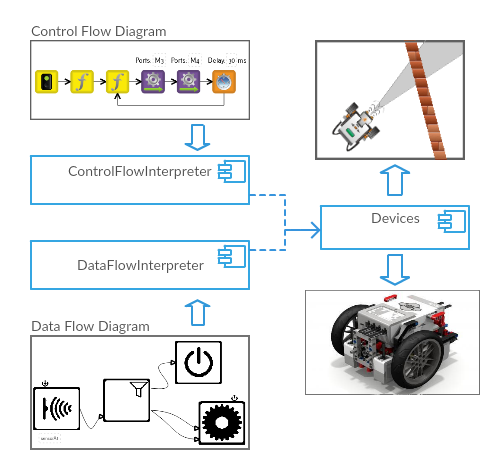
\includegraphics[width=3.5in]{Common.png}
	\caption{The general acrhitecture of the system}
	\label{image:common-architecture}
\end{figure}

\begin{figure}[ht]
	\centering
	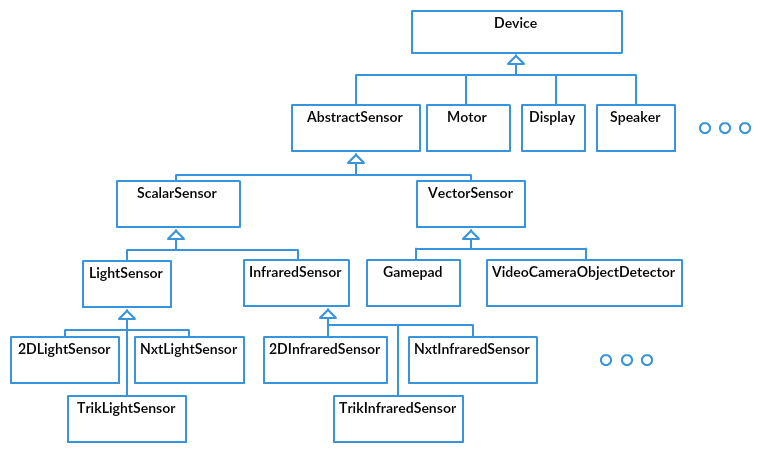
\includegraphics[width=3.5in]{Devices.png}
	\caption{Partial architecture of devices used in dataflow interpreter}
	\label{image:devices-architecture}
\end{figure}

The general acrhitecture of intepreter plugin is presented at fig.~\ref{image:interpreter-architecture}. Given dataflow diagram interpreter traverses, validates and prepares it for interpretation process. For each visited dataflow block implementation object is instantiated. Implementation objects are written in c++. Instantiation is performed by corresponding factory object. Implementation objects are then subscribed each to other like they are connected by flows on diagram, \textit{publish-subscribe} pattern is used here. The set of initial blocks is determined next, those are blocks without incomming flows. After all that done preparation phase is complete and diagram starts beeing interpreted.

\begin{figure}[ht]
	\centering
	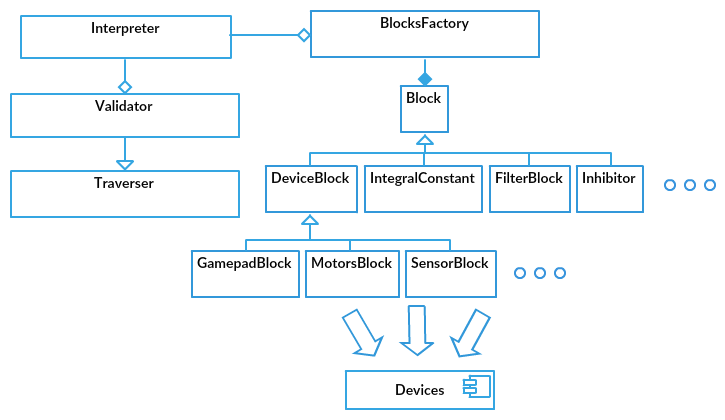
\includegraphics[width=3.5in]{Interpreter.png}
	\caption{The general architecture of dataflow interpreter plugin}
	\label{image:interpreter-architecture}
\end{figure}

Interpretation process is not as straightforward as in most asynchronious dataflow environments. Usually components of dataflow diagram are executed concurrently, on differents threads, processes or even machines (that is actively exploited, for example, by Microsoft Robotics Developer Studio where dataflow diagram is deployed into a number of web-services). That is a pretty convenient way to invoke dataflow diagrams on a powerful hardware, but not a case when we talk about embedded devices. In out case we deal exactly with embedded devices (Lego NXT, EV3, TRIK, Arduino controllers), so we propose here another way of executing dataflow diagrams. The main idea is to intoduce global message queue and event loop for messages processing. When token is published by some block it is enqueued into messages queue and waits for its turn to be delivered to subscribers (fig.~\ref{image:interpreter-interaction}). In fact thus we \textit{flatten} the execution, convert concurrent way of dataflow interpretation to a pseudo-concurrent one where we schedule invocation order on our own. It must be noted that this mechanism is similar to events propagation system of Qt framework. That is actively exploited in our implementation, where message processing is completely performed by $QEventLoop$ class and tokens delivering is done by Qt signal/slot system in $QueuedConnection$ mode. 

Flat execution of dataflow diagram poses a number of small problems, one of them will be discussed here. Input device blocks (for example blocks publishing tokens from ultrasonic sensors) are constantly emitting tokens to subscribers. Subscribers transmit tokens to a next one (possibly in modified state) and so on. Thus there appears a chain of data processing. In out language that chain can activate control flow ports of blocks ``reviving'' them, so the control flow model is implicitly supported in out language (this is important in educational reasons). If later in this chain same input device block will be met then execution will come in a 
counterintuitive way. Such conflicts are ruled out with a simple heruistic that among all the blocks sharing one physical device only one can be active and that is the last activated one. Thus when the execution token comes into some device block it immediately ``deactivates'' conflicting ones. Other problems like messages balancing (in case when some block ``flooding'' the whole messages queue) will not be discussed here.

The last thing we should remark here is the presence of $Fork$ block in our language that usually is not provided by dataflow languages. Flattened model seems to work well on embedded devices, but sometimes users still need to use concurrent execution (for example for executing layers in subsumption architecture). For that reason $Fork$ block is introduced, it forks the execution into a number of platform-specific execution units (for example $pthreads$ on UNIX or $tasks$ on NXT OSEK). This block can be ragarded as low-level control of execution process. It should be also marked that this block almost has no sence in interpretation mode (because execution itself is performed on desktop machine with only sending primitive commands to robot), but will be very useful in future works when autonomous mode will be introduced.

\begin{figure}[ht]
	\centering
	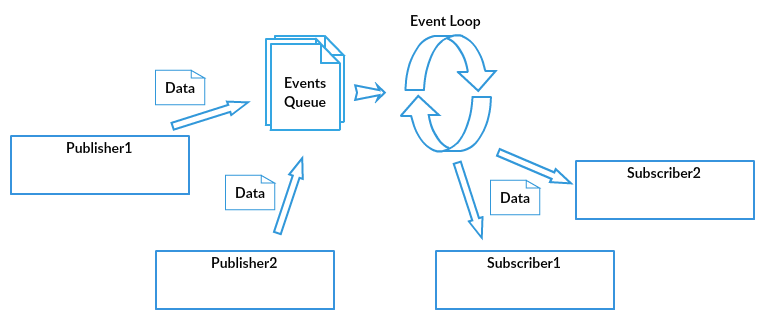
\includegraphics[width=3.5in]{Interaction.png}
	\caption{Proposed mechanism of pseudo-concurrent dataflow interpretation}
	\label{image:interpreter-interaction}
\end{figure}


\section{Conclusion and Discussion}
\label{sec:Conclusion}
In this work we presented the prototype of dataflow language for programming different robotic kits (LEGO MINDSTORMS NXT, LEGO MINDSTORMS EV3, TRIK). The system provides ability to interpret diagrams on 2D- an 3D-simulators and real robotic devices. Proposed an aproach for executing dataflow diagrams on embedded devices. The language implicitly supports control flow model for educational purposes. It is also convenient for expressing typical robotic controllers architectures which is demostrated on example.

The implemented system can be regarded as a platform for future investigations. First of all autonomious mode of work will be implemented. That will be done through code generation into a number of textual languages aready supported by TRIK Studio (NXT OSEK C for Lego, bytecode for EV3, JavaScript, F\#\cite{kirsanov2014robotics} and Kotlin for TRIK). We are also interested in academical research. First of all a formal semantics of our language should be expressed for applying various formal methods of program analysis. Another branch of research will be directed into a DSM-branch, here we want to consider an ability of dynamic langiage metamodel generation from specifications of available modules of robotics middleware (like ROS\cite{quigley2009ros} or Player\cite{gerkey2003player}).

\newpage
\bibliography{IEEEbibl}
\bibliographystyle{IEEEtran}
\end{document}
